\section{Einführung in die Quanteninformatik 2}
\label{sec:einfuehrung-in-die-quanteninformatik-2}

\subsection{Drei Prinzipien des Quanten Computing}
\label{subsec:drei-prinzipien-des-quanten-computing}

Zusammenfassend lässt sich Quanten Computing auf 3 wesentliche Prinzipien herunterbrechen.\\\\
Prinzip 1 - \textbf{Das Quantenregister}: Ein Quantenregister, das aus n-Qubits besteht, wird durch einen $2^n$-dimensionalen Vektorraum über komplexen Zahlen beschrieben.
Der Zustand eines solchen Registers ist eine Überlagerung (Superposition) aller möglichen Basiszustände.
Das bedeutet, dass das Register eine Kombination vieler möglicher Werte gleichzeitig annehmen kann.

Diese Fähigkeit der Superposition ist eine der Hauptstärken von Quantencomputern, da sie es ermöglichen, mehrere Berechnungen parallel durchzuführen.\\

Prinzip 2 - \textbf{Rechenschritte}: Rechenschritte in einem Quantencomputer basieren auf unitären Transformationen.
Diese Transformationen sind umkehrbar, was bedeutet, dass die Berechnung ohne Informationsverlust rückgängig gemacht werden kann.
Jede Operation kann lokal beschrieben werden, wobei nur zwei Qubits gleichzeitig beteiligt sind.

Diese Reversibilität der Rechenschritte stellt einen fundamentalen Unterschied zu klassischen Computern dar, bei denen Informationen während der Berechnung verloren gehen können.\\

Prinzip 3 - \textbf{Messungen}: Misst man den Zustand eines Quantenregisters, so erhält man als Ergebnis einen der Basiszustände mit einer Wahrscheinlichkeit, die aus der Amplitude dieses Zustands abgeleitet werden kann.

Die Messung verändert den Zustand des Systems auf den gemessenen Wert, sodass die ursprüngliche Superposition zerstört wird.\\

In diesen Prinzipien unterscheidet sich das Quanten Computing wesentlich von klassischen Computern.\\


\subsection{Verschränkung}
\label{subsec:verschraenkung}

Eine der interessantesten Eigenschaften von Quantenregistern ist die Verschränkung.
Bei der Verschränkung teilen sich zwei Qubits denselben Zustand.
Das heißt, messen wir den Zustand von Qubit 1, wissen wir auch sofort den Zustand von Qubit 2, ohne dieses gemessen zu haben.
Und was das Ganze noch faszinierender macht: Selbst über große Entfernungen zwischen den verschränkten Qubits bleibt die Eigenschaft der Verschränkung erhalten.
Dies bildet auch die Grundlage für die Quanten-Teleportation, auf die wir später noch zurückkommen.\\

\begin{tcolorbox}[title=Kommentar,
    title filled=false,
    colback=cyan!5!white,
    colframe=cyan!75!black]
    Die Verschränkung war mir bisher ein unbekanntes Konzept, welches sich nur sehr schwer greifen lässt.
    Dementsprechend schwierig war es auch, die Verschränkung zu verstehen und in eigenen Worten zu erklären.
    Besonders, dass diese unabhängig von der räumlichen Entfernung der Qubits erhalten bleibt.\\

    Dazu half mir ein kleines Beispiel: Stellen wir uns zwei Würfel vor, einen roten Würfel und einen blauen Würfel.
    Der blaue Würfel zeigt immer dieselbe Augenzahl wie der Rote.
    Wenn wir nun mit dem Roten würfeln und dieser eine 6 zeigt, wissen wir auch, dass der Blaue eine 6 zeigt, ohne diesen gewürfelt zu haben.
    Und das unabhängig davon, wie weit die beiden Würfel voneinander entfernt sind.
\end{tcolorbox}

Wie erzeugen wir eine solche Verschränkung?
Dazu betrachten wir exemplarisch ein Zwei-Bit-Register $\ket{b_{1}b_{2}}$ im Zustand $\ket{00}$.
Wir wenden auf das erste Bit die Hadamard-Transformation an und anschließend auf beide Bits die Operation CNOT\@.\\
\begin{equation}
    CNOT : \ket{x,y} \rightarrow \ket{x,y\oplus x}
\end{equation}\\

Das ergibt:\\
\begin{align}
    \ket{00} &\xrightarrow{H\otimes I_{2}} \frac{1}{\sqrt{2}}(\ket{0}+\ket{1})\ket{0} = \frac{1}{\sqrt{2}}(\ket{00}+\ket{10}) \\
    &\xrightarrow{CNOT} \frac{1}{\sqrt{2}}(\ket{00}+\ket{11})
\end{align}\\

Wenn wir nun das erste Bit messen, kommt mit einer Wahrscheinlichkeit 50\% das Ergebnis $\ket{0}$ mit dem Folgezustand $\ket{00}$ und mit einer Wahrscheinlichkeit von 50\% das Ergebnis $\ket{1}$ mit dem Folgezustand $\ket{11}$ heraus.
Wir wissen also nach der ersten Messung schon, bevor wir das zweite Qubit überhaupt gemessen haben, wie der Endzustand des Quantenregisters ist.
Und wie bereits zuvor erwähnt, bleibt diese Eigenschaft bei räumlicher Trennung der Qubits erhalten.
Hierbei ist auch zu erwähnen, dass es egal ist, welches der Qubits zuerst gemessen wird oder ob diese überhaupt gleichzeitig gemessen werden.\footnote{\cite[S. 76]{homeister_quantum_2022}}\\
\begin{figure}[H]
    \centering
    \includegraphics[width=0.8\textwidth]{img/Verschränkung Definition}
    \caption{Definition Verschränkung}
    \label{fig:verschraenkung}
\end{figure}

Diesen Zustand nennt man auch Bell-Zustand.
Es gibt insgesamt 4 solcher Bell-Zustände.
Diese beschreiben verschränkte Bits mit einer starken Kopplung (maximal verschränkt).\\
Daraus resultierend gibt es auch Verschränkungen mit einer weniger starken Kopplung.
Ein solcher Zustand könnte beispielsweise so aussehen:
\begin{equation}
    \ket{\phi} = 0.9\ket{00} + 0.1\ket{11}
\end{equation}\\

Hier sind die Qubits auch wieder miteinander verschränkt, allerdings sind die Wahrscheinlichkeiten für die Messergebnisse ungleich verteilt.
Das heißt, wir bekommen mit einer Wahrscheinlichkeit von 90\%, also sehr sicher, den Zustand $\ket{00}$ und nur mit 10\% den Zustand $\ket{11}$, also unsicher.
Diese weniger stark gekoppelten Qubits kommen in der Praxis häufiger vor, etwa durch äußere Einflüsse wie Rauschen oder Dekohärenz auf ehemals maximal verschränkte Qubits.
Das geht mit Leistungseinbußen einher, weshalb versucht wird, den Zustand der maximalen Verschränkung möglichst lange zu erhalten.\\


\subsection{Quantengatter \& Quantenschaltkreise}
\label{subsec:quantengatter-quantenschaltkreise}

„Klassische Schaltkreise bestehen aus Leitungen und Gattern.
Ganz analog bestehen Quantenschaltkreise aus Quantenleitungen und Quantengattern.
Jede Quantenleitung entspricht einem Quantenbit und ein Quantengatter führt eine unitäre Transformation aus.“\footnote{\cite[S. 76]{homeister_quantum_2022}}\\
\begin{figure}[H]
    \centering
    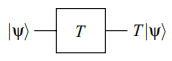
\includegraphics[width=0.35\textwidth]{img/Quantengatter Basic}
    \caption{Quantenschaltkreis}
    \label{fig:quantenschaltkreis}
\end{figure}

Wenn wir eine Berechnung mit mehreren Qubits ausführen, ergibt sich der Endzustand $\ket{x, y, z}$ aus dem Tensorprodukt der einzelnen Gatter\footnote{\cite[S. 76]{homeister_quantum_2022}}:
\begin{equation}
    (I_{2} \otimes W \otimes I_{2})(U \otimes V)\ket{x, y, z}
\end{equation}

\begin{figure}[H]
    \centering
    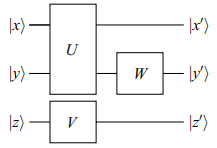
\includegraphics[width=0.35\textwidth]{img/Quantengatter 3er}
    \caption{Quantenschaltkreis mit Tensorprodukt}
    \label{fig:quantenschaltkreis-tensorprodukt}
\end{figure}

Da bei Quantenschaltkreisen die Umkehrbarkeit der Berechnungen garantiert werden muss, ist die Summe der Eingabe-Qubits = Summe der Ausgabe-Qubits und pro Gatter dürfen höchsten 3 Qubits einbezogen werden.
Um dies zu gewährleisten, nutzen wir das Toffoli-Gatter, welches im nächsten Kapitel erläutert wird.
Außerdem können Qubits nicht kopiert werden, deshalb dürfen sich die Quantenleitungen nicht verzweigen und das Ergebnis eines Gatters nicht mehrfach verwendet werden.
Auf den Grund dafür kommen wir später nochmal zurück.\\

Eine der wichtigsten Operationen in der Quanteninformatik ist die Negation, genauer die kontrollierte Negation CNOT\@.
Dieses Gatter wird für alle Quantenoperationen benötigt, so zum Beispiel bei der Verschränkung.
Darstellen lässt es sich wie folgt:
\begin{equation}
    CNOT : \ket{x,y} \rightarrow \ket{x,y\oplus x}
\end{equation}

oder als Matrix:
\begin{equation}
    CNOT =
    \begin{pmatrix}
        1 & 0 & 0 & 0 \\
        0 & 1 & 0 & 0 \\
        0 & 0 & 0 & 1 \\
        0 & 0 & 1 & 0
    \end{pmatrix}
\end{equation}

Dieses CNOT-Gatter negiert nur dann das zweite Qubit, wenn das erste Qubit im Zustand $\ket{1}$ ist.\\

Weitere wichtige Operationen sind die Hadamard-Transformation, die wir bereits kennen, sowie die Pauli-Matrizen.
Die Pauli-Matrizen negieren ebenfalls, mithilfe einer unitären Transformation auf einem Bit.
Die bekannteste ist der „Bitflip“ X:\footnote{\cite[S. 79]{homeister_quantum_2022}}
\begin{equation}
    X =
    \begin{pmatrix}
        0 & 1 \\
        1 & 0
    \end{pmatrix}
\end{equation}

Die zwei weiteren Pauli-Matrizen sind der „Phasenflip“ Z:
\begin{equation}
    Z =
    \begin{pmatrix}
        1 & 0 \\
        0 & -1
    \end{pmatrix}
\end{equation}

und der „Y-Flip“ Y:
\begin{equation}
    Y =
    \begin{pmatrix}
        0 & -i \\
        i & 0
    \end{pmatrix}
\end{equation}

\begin{figure}[H]
    \centering
    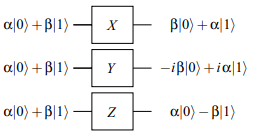
\includegraphics[width=0.5\textwidth]{img/Quantengatter Pauli_Matrizen}
    \caption{Pauli-Matrizen}
    \label{fig:pauli-matrizen}
\end{figure}

Durch die Kombination dieser drei Gatter CNOT, Hadamard-Transformation, sowie Pauli-Matrizen lassen sich alle Quantenberechnungen abbilden.
Sie bilden die grundlegendsten Rechenoperationen eines Quantencomputers.
Mit einem wesentlichen Unterschied zu logischen Gattern: bei diesen lässt sich der Endzustand nicht unbedingt wieder in den Anfangszustand überführen.
Bei Quantengattern ist dies eine zwingende Voraussetzung, sie müssen umkehrbar sein.\\


\subsection{Umkehrbare Berechnungen}
\label{subsec:umkehrbare-berechnungen}

Wie bereits zuvor erwähnt, muss jede Rechenoperation eines Quantencomputers umkehrbar sein.
Es dürfen also keine Informationen gelöscht werden, wie es beispielsweise bei der Anwendung einer logischen AND-Operation passiert: aus zwei Eingabewerten wird ein Ausgabewert kombiniert.
So folgt aus 1 AND 0 = 0, jedoch ebenfalls aus 0 AND 0 = 0.
Sehen wir den Endzustand 0, wissen wir also nicht, welchen Zustand die beiden Bits zu Beginn hatten.
Das bedeutet, wir können Quantenrechenprozesse nicht auf dieselbe Art verarbeiten wie klassische Rechenprozesse.\\

Allerdings kann jede klassische Operation in eine umkehrbare Operation umgewandelt werden.
Veranschaulichen wir uns dies anhand des Toffoli-Gatters.\\

Das Toffoli-Gatter ist ein universelles, umkehrbares Gatter, welches AND, OR und NOT Operationen ersetzen kann.
Es besteht aus drei Eingabebits a, b, c und drei Ausgabebits a, b und $c\oplus(a\land b)$:\footnote{\cite[S. 87]{homeister_quantum_2022}}\\
\begin{figure}[H]
    \centering
    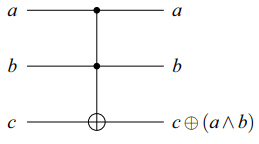
\includegraphics[width=0.35\textwidth]{img/Umkehrbare_Berechnungen Toffoli}
    \caption{Toffoli-Gatter}
    \label{fig:toffoli-gatter}
\end{figure}

Exemplarisch für AND: Wollen wir zum Beispiel ein Bit negieren, mit der Eingabe (a, b, c) = (1, 1, 0).
Dann ergibt die Rechnung über das Toffoli-Gatter (1, 1, 1), denn $(1\land 1) \oplus 0 = 1$.
Hier ist nun auch zu sehen, dass die Berechnung umkehrbar ist, wenn wir die Schritte einmal rückwärts gehen.
Dies ist genauso für die anderen Operatoren möglich, bedarf gegebenenfalls nur Umformung und den Einsatz mehrerer Toffoli-Gatter.\\

Auf diese Weise können wir jede klassische Rechenoperation umkehrbar gestalten, sodass diese auch für unsere Quantenschaltkreise nutzbar sind.\\


\subsection{Gestörte Berechnungen}
\label{subsec:gestoerte-berechnungen}

Wie wir bisher sehen konnten, scheint alles, was wir mit klassischen Computern berechnen, genauso effizient mit Quantencomputern berechenbar.
Warum also steht nicht bei jedem ein Quantenrechner zu Hause (wenn wir die Kosten mal außen vor lassen)?\\

Einer der Gründe dafür ist die Fehleranfälligkeit.
Während klassische Bits die Zustände 0 oder 1 abbilden, können Quantenbits bis zur Messung $\ket{0}$ oder $\ket{1}$ oder beide Zustände gleichzeitig annehmen.
Verdeutlichen wir, was das in der Praxis bedeutet: Nehmen wir an, der Zustand 0 eines klassischen Bits wird durch 0V und der Zustand 1 durch 5V dargestellt.
Nun kann es zu Spannungsschwankungen kommen und wir geben 4V statt 5V\@.
Da wir aber keinen Zustand für 4V haben, aber nur 2 Zustände abbilden können, können wir auch sagen, der Zustand 0 wir durch eine Spannung <2,5V abgebildet und der Zustand 1 durch >2,5V.
So liefert der Rechner uns auch weiterhin ein zuverlässiges Ergebnis, trotz Störung.\\

Die ist allerdings nicht für Quantenbits möglich, da wir nicht nur diese zwei Zustände abbilden.
Was bedeutet also hier eine Spannungsschwankung von 5V auf 4V?
Das wissen wir nicht, da bis zur Messung der Zustand nicht feststeht, so können wir also auch kein zuverlässiges Ergebnis mehr liefern.
So können selbst kleinste Störungen Quantenberechnungen verfälschen.
Zu beachten ist, dass bei einem gestörten Quantengitter sich der Fehler nur addiert.
Das heißt, der Fehler eines Gatters bleibt zwar in weiteren Berechnungen erhalten, jedoch wird er nicht größer.\\

Würden wir zum Beispiel ein Qubit durch 3 Quantengatter nacheinander umformen, wobei jedes dieser Gatter einen Fehler von 2\% hinzufügt, so beträgt der Fehler des Endzustands 6\%.
Das heißt, bei 50 Quantengattern welche einen Fehler von 2\% hinzufügen, beträgt der Fehler des Endzustands 100\%.
Wenn die Fehler nun aber exponentiell wachsen würden, hätten wir nach 3 Gattern einen Fehler von 8\%, nach 50 Gattern (theoretisch) einen Fehler von $2^{50}$\%.\\

Um die Frage vom Beginn des Kapitels nochmal aufzunehmen: Einer der Gründe weshalb nicht jeder einen Quantencomputer zu Hause stehen hat, ist die Fehleranfälligkeit der Berechnungen.
Es bedarf großen Aufwands solche Fehler zu vermeiden und zu korrigieren.\\


\subsection{Grenzen}
\label{subsec:grenzen}

Angenommen in 10 Jahren ist das Problem der Dekohärenz gelöst, werden Quanten Computer die Lösung aller mathematischen Probleme sein?
Obwohl Quanten Computing noch mitten in der Entwicklung stecken, lässt sich jetzt schon absehen: Die Antwort darauf ist „Nein“.\\

\subsubsection{NP-vollständige Probleme}
\label{subsubsec:np-vollstaendige-probleme}
Eine der zentralen Fragen der Komplexitätstheorie beschäftigt sich mit NP-vollständigen Problemen.
Sie beschreibt Probleme, welche sich zwar leicht überprüfen lassen, doch algorithmisch mindestens eine exponentielle (O($2^{n}$), häufig sogar fakultative (O(n!)) Laufzeit haben.
Und würde man für ein NP-vollständiges Problem eine Lösung finden, also ein Algorithmus mit polynomieller O($n^{x}$) Laufzeit, so könnten alle dieser Probleme darauf umgeformt und gelöst werden.\\

Doch selbst Quantencomputer scheinen keine Lösung für diese Probleme finden zu können.
Das liegt daran, dass selbst Quantenalgorithmen, wie etwa der bekannte Shor-Algorithmus (zur Faktorisierung großer Zahlen),
oder der Grover-Algorithmus (zur unstrukturierten Suche in Datenbanken), zwar eine deutliche Geschwindigkeitsverbesserung im Vergleich zu klassischen Algorithmen bieten,
jedoch keine exponentielle Reduktion der Komplexität bei NP-vollständigen Problemen ermöglichen.\footnote{\cite[S. 165]{homeister_quantum_2022}}\\
Hier stoßen Quantencomputer also auf dieselben grundlegenden Herausforderungen wie klassische Computer.\\

\begin{tcolorbox}[title=Kommentar,
    title filled=false,
    colback=cyan!5!white,
    colframe=cyan!75!black]
    Wir hatten zunächst überlegt, den Grover- oder Shor-Algorithmus genauer zu beleuchten, haben uns dann aber dagegen entschieden,
    da wir uns auf die Grundlagen des Quanten Computing konzentrieren und uns nicht in einem komplexen Algorithmus verlieren wollten.\\

    Als wir mit dem Thema und der Recherche zur Quanteninformatik begonnen haben, war mir nicht bewusst, dass selbst Quantencomputer,
    welche noch in den Anfängen stecken und ein großes Potenzial bieten, schon jetzt an Grenzen stoßen, wie bei den NP-vollständigen Problemen.
    Es ist faszinierend zu sehen, dass selbst Quantencomputer, eine Technologie die man sonst nur aus Sci-Fi Serien kennt, nicht alle mathematischen Probleme lösen kann.
\end{tcolorbox}

\subsubsection{Die perfekte Uhr}
\label{subsubsec:die-perfekte-uhr}
Ein weiteres Problem, auf welches Quantencomputer stoßen werden, ist die perfekte Zeitmessung, also die perfekte Uhr.
Jede Uhr hat zwei fundamentale Eigenschaften: Präzision und Zeitauflösung.
Die Zeitauflösung gibt an, wie klein die messbaren Zeitintervalle sind (also wie oft die Uhr tickt) und die Präzision gibt an, mit welcher Ungenauigkeit bei jedem Tick zu rechnen ist.
Ein Forscherteam hat gezeigt, dass es unmöglich ist gleichzeitig die perfekte Präzision und die perfekte Zeitauflösung zu erreichen.\\

Warum ist das wichtig für das Quanten Computing?
Aktuell haben Quantencomputer noch mit anderen Problemen, wie etwa der Dekohärenz oder Ungenauigkeiten bei den verwendeten Bauteilen zu kämpfen.
Allerdings zeigen Rechnungen, dass man nicht mehr so weit davon entfernt ist, bis die physikalische Grenze der Zeitrechnung die nächste Limitation für Geschwindigkeit und Zuverlässigkeit darstellt.\footnote{\cite{tuwien_grenzen_2023}}\\\\

\begin{tcolorbox}[title=Kommentar,
    title filled=false,
    colback=cyan!5!white,
    colframe=cyan!75!black]
    An der Stelle nur ein kleiner Ausblick auf die perfekte Uhr.
    Da ich bei meiner Recherche schnell in der Thermodynamik und Quantenmechanik gelandet bin und es ein umfangreiches physikalisches Wissen voraussetzt, vertiefe ich die perfekte Uhr nicht weiter.
\end{tcolorbox}


\subsection{Zukunft}
\label{subsec:zunft}

Wie sieht die Zukunft des Quanten Computing aus?
Was sind oder werden Anwendungsgebiete für diese Technologie sein?\\

\subsubsection{Quantum Machine Learning}
\label{subsubsec:quantum-machine-learning}
Künstliche Intelligenz oder auch Machine Learning sind zwei der Bereiche, in denen Quantencomputer eine große Rolle spielen könnten.
So schreibt die Fraunhofer-Allianz Big Data und Künstliche Intelligenz: \("\)Verfahren der künstlichen Intelligenz und des Machine Learnings lassen sich für Quantencomputer so anpassen, dass sie mehrere Lösungswege gleichzeitig beschreiten können.
Damit können Quantencomputer große Datenbestände in einem einzigen Schritt verarbeiten, Muster in den Daten aufspüren, die klassische Computer nicht entdecken und auch auf unvollständigen oder unsicheren Daten verlässliche Ergebnisse liefern.\("\)\footnote{\cite{tuwien_grenzen_2023}}
Quantencomputer könnten also die Lernverfahren von KI deutlich beschleunigen und verbessern.\\

Dies birgt allerdings auch ein Risiko, dessen ist sich auch das Bundesamt für Sicherheit in der Informationstechnik bewusst und gab in Kooperation mit Capgemini und dem Fraunhofer-Institut für Intelligente Analyse- und Informationssysteme eine Studie in Auftrag, die Quantum Machine Learning (QML) im Kontext von IT-Sicherheit untersuchen soll.\footnote{\cite{BSI_QUITS_2022}}
So hat QML beispielsweise großes Potenzial für die Malware und Spam Erkennung, sowie Kryptografie.
Gleichzeitig weiß man jetzt schon, dass aktuelle Verschlüsselungsmethoden, wie RSA oder ECC, durch Quantencomputer gebrochen werden können.
Daher wird bereits an quanten-resistenten Verschlüsselungsmethoden gearbeitet.\footnote{\cite{BSI_quantum_2022}}\\

\begin{tcolorbox}[title=Kommentar,
    title filled=false,
    colback=cyan!5!white,
    colframe=cyan!75!black]
    Die Studie des BSI ist tatsächlich sehr interessant zu lesen.
    Sie ist zwar von 2022, aber gibt einen guten Überblick über die Möglichkeiten und Risiken von Quantum Machine Learning.
\end{tcolorbox}

\subsubsection{Simulationen}
\label{subsubsec:simulationen}
Die Simulation von chemischen Molekülen.
Etwas bei dem selbst Supercomputer an ihre Grenzen stoßen.
Erstaunlicherweise ist die detaillierte Simulation von etwas so Kleinem wie Molekülen eine der größten Herausforderungen für unsere modernen Computer.
Hier könnten Quantencomputer Unterstützung leisten.
So schreibt das Fraunhofer Cluster of Excellence Cognitive Internet Technologies:
\("\) Mithilfe der Simulation von Molekülen könnten in Zukunft beispielsweise gezielt Katalysatoren entwickelt werden, die chemische Produktionsverfahren effizienter machen.
Chancen ähnlicher Größenordnung ergeben sich für die Pharmaindustrie.
Auch Forschung zu den im Angesicht des Klimawandels besondere relevanten Batterien zählt zum Anwendungsbereich der Simulation.\("\)\footnote{\cite{Fraunhofer_quantencomputing_2025}}
Deshalb erforscht das deutsche Zentrum für Luft- und Raumfahrt (DLR) zusammen mit dem Fraunhofer-Institut für Werkstoffmechanik IWM unter Verwendung des IBM-Quantencomputers neue Wege des Materialdesigns.\footnote{\cite{FraunhoferIWM_quantencomputer_2025}}\\

Neben den genannten Anwendungsgebiete wird außerdem ein Nutzer in der Logistik (optimaler Verteilung begrenzter Ressourcen), den Ingenieurswissenschaften und dem Finanzwesen (Risikoanalysen und Optimierung von Portfolios) gesehen.\footnote{\cite{Fraunhofer_quantencomputing_2025}}\\








